\section{Rollout-to-Scorer Distillation}
\label{sec:method}
\label{sec:repairs}
\label{sec:repairs-r2s}

\method{} targets the rollout--scorer gap of \Cref{sec:gap}. The teacher's rollouts from the student's states carry the judgment its scores lack. As illustrated in \Cref{fig:pipeline}, we therefore let the teacher take over from those states, read off the scores it gives with its own ending in view, and fine-tune it to give those scores closed-book, with no takeover in context; the refrozen teacher then scores ordinary OPD. The student never sees a takeover.

\begin{figure}[t]
\centering
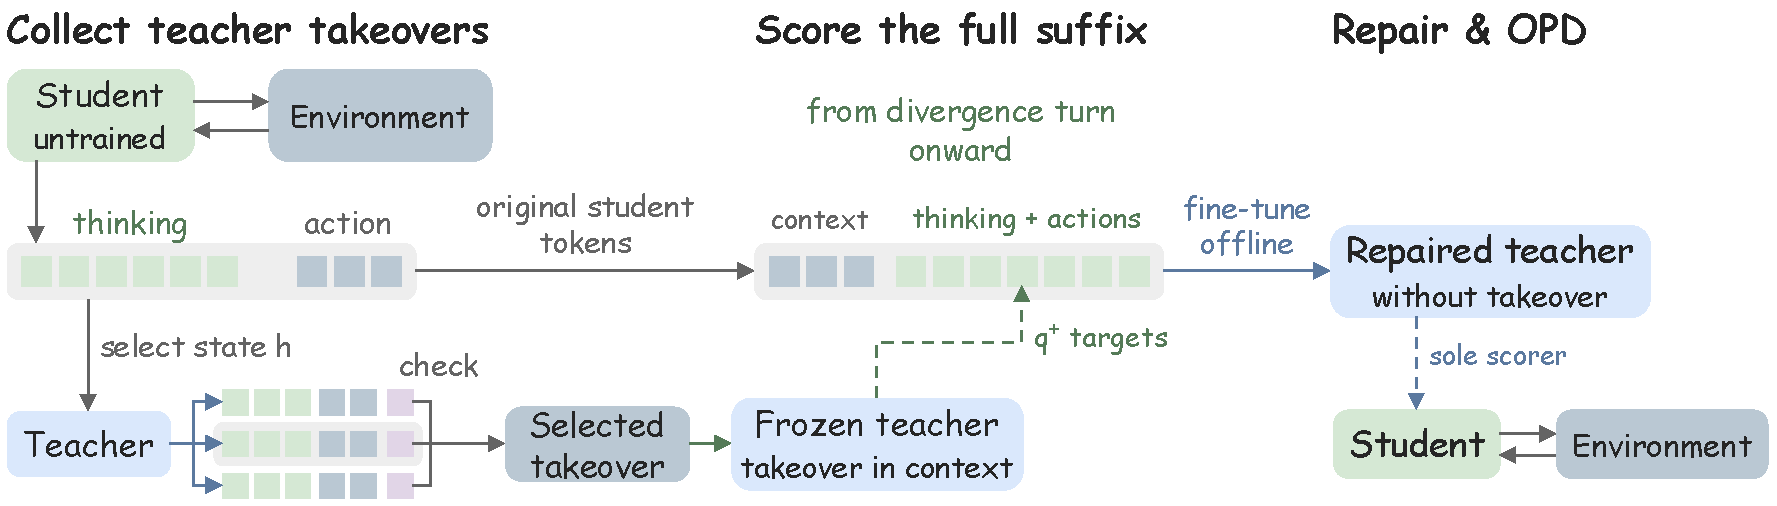
\includegraphics[width=\linewidth]{figures/fig3_method.pdf}
\caption{\textbf{\method{} repairs the teacher's scores on the full assistant suffix before ordinary OPD.} With a selected takeover from the untrained student's state in context, the frozen teacher $T_0$ scores the student's thinking and actions from the divergence turn onward ($q^{+}$). A copy learns these targets without the takeover and becomes the sole OPD scorer.}
\label{fig:pipeline}
\end{figure}


\textbf{The teacher takes over where the student departs most from it.} We first let the untrained student play the training tasks. In each of its episodes we mine the divergence turn: the turn where the student's thinking departs most from the teacher's, measured by OPD's own per-token divergence averaged over that thinking,
\begin{equation}
\label{eq:divscore}
\Delta_t=\frac{1}{|\thinkspan_t|}\sum_{i\in\thinkspan_t}
\left[\log \student(y_{t,i}\mid h_t,y_{t,<i})-\log T_0(y_{t,i}\mid h_t,y_{t,<i})\right],
\end{equation}
where $\thinkspan_t$ is the thinking of turn $t$, the part of $y_t$ before the action, and $T_0$ is the original teacher; the divergence turn has the largest $\Delta_t$. Only the thinking is compared, because it decides the action that follows. From the state at each mined turn, the teacher takes over $K$ times and plays the episode to its end. The choice among these takeovers is general: any check that tells a finishing takeover from a failing one will do, such as consensus among the takeovers, an LLM-as-a-judge, or the ground truth, which is the task's own 0--1 reward. Consensus and a judge need no reward, so \method{} can also run where no reward is available. A state is kept when at least $m$ of its takeovers pass the check, and the shortest of them is selected as $\tau_h$.

\textbf{The judgment supervises the complete suffix from the divergence state.}
For a kept state $h$, the frozen teacher $T_0$ scores the rest of the student's own episode, every token of its thinking and actions from $h$ to the end, with the takeover $\tau_h$ in context. These informed scores are the targets $q^+$. The takeover only informs them; its tokens never replace the student's. A trainable copy $T_\phi$ sees the same episode without the takeover and learns to give the same scores:
\begin{equation}
\label{eq:r2s}
\mathcal{L}_{\mathrm{R2S}}(\phi)=
\mathbb{E}_{h}\,\mathbb{E}_{h'}\Big[\mathrm{CE}\big(\underbrace{T_0(\cdot\mid\tau_h,h')}_{q^{+}},\;T_\phi(\cdot\mid h')\big)\Big],
\end{equation}
where $h'$ runs over the student's histories from $h$ to the end of its episode, one per token the student wrote, and $\mathrm{CE}$ is the cross-entropy. Refrozen, $T_\phi$ is an ordinary next-token scorer, and OPD uses it in place of $T_0$.
